\documentclass[withoutpreface]{cumcmthesis}
\usepackage[framemethod=TikZ]{mdframed}

\hypersetup{
    hidelinks,
    colorlinks=true,
    allcolors=black,
    pdfstartview=Fit,
    breaklinks=true
}

\title{寻找惯性传感器运动数据中的“指纹”}

\begin{document}

\crefname{subsection}{小节}{小节}

\maketitle

\begin{abstract}
MEMS 惯性传感器的发展使得通过运动姿态进行身份识别成为可能,其中如何从运动数据中提取出有效的特征并进行分类是一个重要的问题。
本文面临的问题是在只有少量已知类别的样本的情况下,设计模型判断任意来自 2 个未知类别的运动数据是否来自同一人。

本文从化学实验中的纸层析法和刑侦中的指纹鉴定,
原创性地提出了为运动数据绘制“指纹图谱”的方法。

在构建模型阶段,对参考数据集的原始时间序列进行卡尔曼滤波处理后,
对每个测量对象(X, Y, Z 轴加速度/角速度)提取出 8 种有量纲指标(最值、均值、方差等),
以类似“层析”的方式呈现为图表。
随后,本文建立了一套评价标准,对这 $6 \times 8 = 48$ 种特征进行评估,
并筛选出了最能够反映数据来自同一个人或者不同的人的 12 个特征,
作为下一步测试数据集的判断依据。

在问题求解阶段,对测试数据集的每一对样本提取出 12 项特征后,
将其分别显示在 12 条“滤纸条”上,即得到了该数据的“指纹”。
直观地看,如果该数据对的指纹非常相似,则判断该数据对来自同一名志愿者;如果指纹相差非常大,则判断该数据对来自不同的志愿者。
在实验中,我们使用余弦相似度的方法,通过计算每一对 12 维向量的余弦相似度,
并线性映射为 $[0, 1]$ 区间上的相似概率,以此判断其是否来自同一名志愿者。

本文使用参考数据集进行置信阈值的确定和准确性验证,最终本模型以参考数据集进行的测试正确率为 87.08\%。
最终以该模型得到的判断结果中,测试数据对有 52 对被判断为身份一致,48 对被判断为身份不一致。

\keywords{惯性传感器\quad 卡尔曼滤波\quad 时域信号特征\quad 余弦相似度}

\end{abstract}

\tableofcontents

\newpage

\section{问题重述}

身份识别在数字领域的重要性随着社会发展正在不断增加,然而传统的认证方法例如密码和验证码在今天安全性已变得非常低;
生物识别技术例如人脸、指纹、声纹识别虽已得到推广,但也存在被窃取和伪造的风险。

除了人脸、指纹等静态的生物特征,有人提出了基于运动特征的生物识别方法,例如步态识别,已被证明具有相当的独特性,并且不易被盗取。
MEMS 惯性传感器(IMU)是常用于记录运动状态的传感器,通过记录自身的三轴加速度及旋转角速度可以还原自身的空间运动状态,并且使用成本非常低,因此有望用于实现新的运动生物识别。

问题首先给出了由 10 名志愿者手握惯性传感器在空中书写符号时记录下的传感器数据,这 10 名志愿者作为“已知类别”。
参考数据的采样频率为 500 Hz。
问题另外给出了从 16 名其他志愿者采集的 200 份运动数据(采样频率为 100 Hz),随机两两配对组成 100 个样本对,要求设计模型实现对这 100 个样本对的身份一致性识别,也就是说,判断每一对数据是否来自同一个人。

\section{问题分析}

本问题与常规识别问题的不同在于,它并非要求将给出的测试数据归到一个已知的类别中(例如从图片中识别文字),而是基于少量的已知类别样本判断任意两个未知类别样本是否属于同一个个体,并且这两个样本根本不属于之前已知的任一个体。
这就好比给出一些来自未知语言的文字,要求在并不知道这些文字含义的情况下判断任意两个文字是否来自同一门语言。

经过论证,以下两种方案是不可行的:

\begin{enumerate}
    \item 重建运动轨迹,并根据轨迹进行相似度的判断。\\
    理由:IMU 记录的是加速度,即位移对时间的二阶导数,在缺少初值的情况下,通过二重积分得到的轨迹没有任何意义。
    除此之外,从数据集可以发现不同样本的大小是不同的,也就是说每次实验时完成的动作是不同的,这进一步增大了轨迹比较的难度。
    \item 让参考数据集中的每一名志愿者代表一类人,基于参考数据建立一个具有 10 种运动姿势的库,将测试数据分到这些类别中判断是否来自同一类。\\
    理由:测试数据集来自 16 名志愿者,如果只将人分为 10 种,根据抽屉原理,必然有至少 2 个人被划分到同一类中,这会极大降低识别的准确度。
\end{enumerate}

基于该问题的背景和条件,判断一个样本对是否来自同一个体,本质上是寻找两组数据之间是否存在相似的特征。

要想比较两组数据的相似程度,最直接的办法是使用一些分类器对时间序列直接进行比对,例如 K-近邻算法(KNN)。
但是需要注意的是,本题目中给出的运动数据所记录的并非相同的动作——每个志愿者在自己的 10 次实验中完成的动作是不一样的,
这就导致分类器的输出会将不同的人做出的相似的动作划分到同类,而不是将同一个人的各种动作划分到同一类中。
因此 KNN 算法并不适用于本题目。

由此我们可以得出,用于进行比较的不应该是时间序列本身,而是从时间序列中提取出的\textbf{数字特征}。

我们希望从每一组数据中提取出一些特征,使得来自同一名志愿者的数据特征相似,而来自不同志愿者的数据特征差异较大,
并且构建一种方法,通过它将任意两组数据的特征进行比较,从而判断它们是否来自同一个人。

一种可行的办法是训练孪生神经网络(Siamese Neural Network, SNN)对数据进行比较。
孪生神经网络的结构非常适合判断未知数据的相似程度,例如两张人脸的图片。
但是神经网络的训练需要大量的数据,而本题目中给出的数据量较少,不一定能保证模型的准确度,
并且我们无法得知神经网络是如何判断两组数据的相似度的,这就无法保证模型的可解释性。
因此本文在尝试后将其放弃。

最终,本文从化学实验中的纸层析法和刑侦中的指纹鉴定中获得灵感,通过绘制出特征数据的“指纹图谱”寻找出最能够区分人运动特征的若干组特征,
再利用这些特征判断测试数据集中的各个样本对的身份一致性。

\section{模型假设}

为了简化问题及求解过程,本文提出以下假设:
\begin{enumerate}
    \item 至少前 10 名志愿者使用的手机传感器是相同的(精度、采样频率),且后 16 名志愿者使用的手机传感器也是相同的。
    \item 实验采用的 MEMS 传感器性能足够好,记录下来的数据都是有效的。
\end{enumerate}

\newpage

\section{符号及变量说明}

\begin{table}[!htb]
    \centering
    \begin{tabular}{cc|cc}
    \toprule[1.5pt]
        符号 & 含义 & 符号 & 含义 \\
    \midrule[1pt]
        $x_{max}, x_{min}$ & 时域信号的最大值/最小值 & $x_{mid}$ & 时域信号的中位数 \\
        $\mu$ & 时域信号的均值 & $\sigma^2$ & 时域信号的方差 \\
        $x_{peak}$ & 时域信号的峰值 & $x_{p-p}$ & 时域信号的峰-峰值 \\
        $x_{rms}$ & 时域信号的有效值 & $C$ & 时域信号的峰值因子 \\
        $C_e$ & 时域信号的裕度因子 & $I$ & 时域信号的脉冲因子 \\
        $S_f$ & 时域信号的波形因子 & $K$ & 时域信号的峭度因子 \\
        $S_k$ & 时域信号的偏斜度 & $K_1$ & 第 1 项评估指标 \\
        $K_2$ & 第 2 项评估指标 & $K$ & 总评估指标 \\
        $\cos \theta$ & 余弦相似度 & $P$ & 相似概率 \\
        $P_t$ & 置信阈值 & & \\
    \bottomrule[1.5pt]
    \end{tabular}
\end{table}

\section{模型的建立与求解}

\subsection{数据预处理}

本文首先对数据进行了简单的评估和预处理。

\subsubsection{初步统计分析}

我们首先使用折线图直观了解数据随时间变化的情况。
\cref{fig:reference-1-4} 是根据参考数据集中志愿者 1 的第 4 次实验绘制出的加速度和角速度时间序列图。
从中可以看出,在整个动作采集的过程中,加速度和角速度随时间变化的曲线总体较为平滑,但在局部仍然存在毛刺和抖动的问题。

\begin{figure}[!htbp]
    \centering
    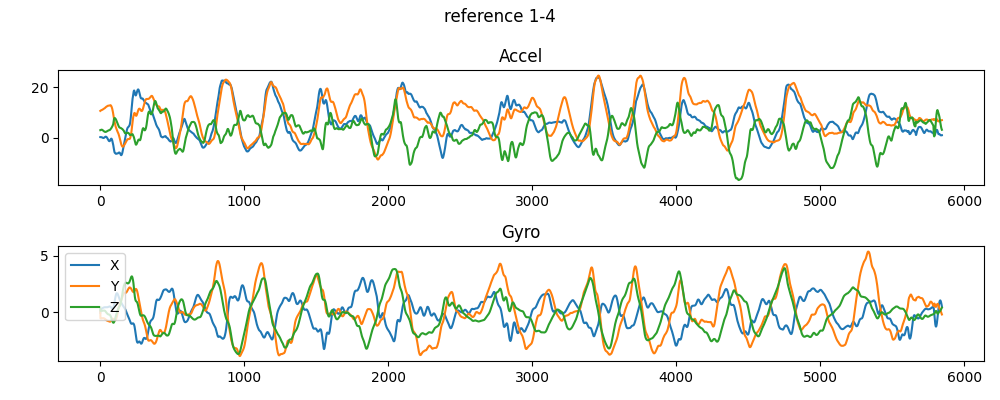
\includegraphics[width=\textwidth]{figures/reference-1-4.png}
    \caption{参考数据 1-4 时间序列}
    \label{fig:reference-1-4}
\end{figure}

\cref{fig:reference-1-4-boxplot} 是根据参考数据集中志愿者 1 的第 4 次实验绘制出的加速度和角速度箱型图。
可以发现,某些类别存在一定数量的离群点。

\begin{figure}
    \centering
    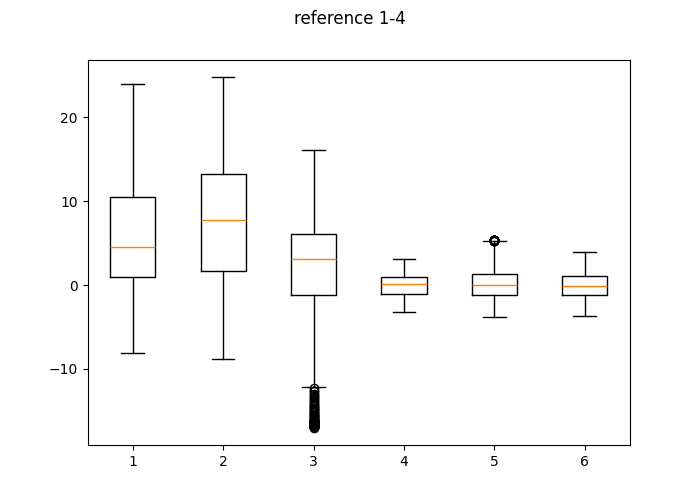
\includegraphics[width=0.7\textwidth]{figures/reference-1-4-boxplot.png}
    \caption{参考数据 1-4 箱型图}
    \label{fig:reference-1-4-boxplot}
\end{figure}

本文对来自其余的志愿者的数据进行了同样的分析,得到的结论是一致的。
这说明本问题的数据来源较为可靠,但仍需要进行过滤处理。

\subsubsection{使用卡尔曼滤波处理数据}

为了优化 MEMS 的传感器原始数据,本文采用广泛用于惯性传感器的卡尔曼滤波算法对其进行处理。

\cref{fig:Kalman}是对参考数据集志愿者 1 的第 2 次实验 X 轴加速度进行卡尔曼滤波前后的对比展示,可以看出滤波后的数据比滤波前明显有更少的抖动。

对于参考数据集其余的所有样本,本文采用相同的参数统一进行卡尔曼滤波处理。

\begin{figure}[!htbp]
    \centering
    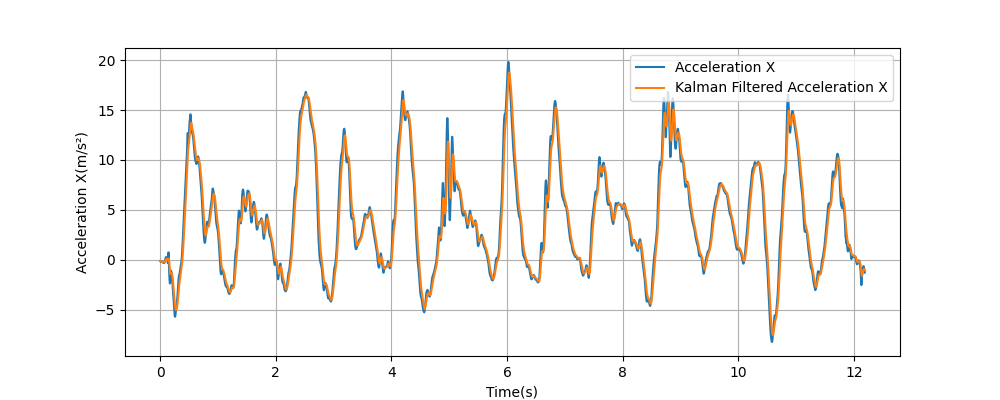
\includegraphics[width=\textwidth]{figures/kalman.png}
    \caption{卡尔曼滤波效果示例}
    \label{fig:Kalman}
\end{figure}

\subsection{IMU 数据特征提取}
\label{imu_features_extraction}

\subsubsection{时域信号的特征提取}
\label{features_extraction}

对于惯性传感器数据这样的时域信号,我们需要提取出它的一些特征(统计指标),用于后续的比较。

统计指标包含有量纲指标和无量纲指标,
本文尝试了对滤波后的参考数据提取 8 种有量纲指标(见\cref{chart:features_dimension})
和 6 种无量纲指标(见\cref{chart:features_dimensionless}) \cite{1021136457.nh}。

\begin{table}[!htbp]
\centering
\caption{时域信号的几种有量纲指标}
\begin{tabular}{|l|l|}
\hline
\multicolumn{1}{|c|}{名称} & \multicolumn{1}{c|}{表达式} \\ \hline
最大值/最小值 & $x_{max}, x_{min}$  \\ \hline
均值 & $\mu$  \\ \hline
中位数 & $x_{mid}$ \\ \hline
方差 & $\sigma^2$ \\ \hline
峰值 & $x_{peak} = \max(|x_{min}|, |x_{max}|)$ \\ \hline
峰-峰值 & $x_{p-p} = x_{max} - x_{min}$ \\ \hline
有效值 & $x_{rms}$ \\ \hline
\end{tabular}
\label{chart:features_dimension}
\end{table}

\begin{table}[!htbp]
\centering
\caption{时域信号的几种无量纲指标}
\begin{tabular}{|l|l|l|}
\hline
\multicolumn{1}{|c|}{名称} & \multicolumn{1}{c|}{表达式} & \multicolumn{1}{c|}{含义} \\ \hline
峰值因子 & $C = \frac{x_{peak}}{x_{rms}}$ & 信号峰值与有效值(RMS)的比值 \\ \hline
裕度因子 & $C_e = \frac{x_{peak}}{x_r}$ & 信号峰值与方根幅值的比值 \\ \hline
脉冲因子 & $I = \frac{x_{peak}}{x_{arv}}$ & 信号峰值与整流平均值(绝对值的平均值)的比值 \\ \hline
波形因子 & $S_f = \frac{x_{rms}}{x_{arv}}$ & 有效值(RMS)与整流平均值的比值 \\ \hline
峭度因子 & $K = \frac{\mu_4}{\sigma^4}$ & 四阶中心矩与标准差的四次方的比值 \\ \hline
偏斜度  & $S_k = \frac{\mu_3}{\sigma^4}$ & 三阶中心矩和标准差的三次方的比值,与峭度类似 \\ \hline
\end{tabular}
\label{chart:features_dimensionless}
\end{table}

\subsubsection{特征数据的可视化}

为了将同一名志愿者的每次运动,以及不同志愿者的所有运动的某一项数字特征进行直观比较,
本文将所有参考数据的每一项特征绘制成类似于纸层析中的"滤纸条“的形式,表现如\cref{fig:滤纸条} 所示。
其中横轴代表从 1 到 10 的实验次数,每一种颜色代表来自一名志愿者,每一个点代表该志愿者某一次实验的该项特征值。

\begin{figure}[!htbp]
    \centering
    \begin{minipage}[c]{0.48\textwidth}
        \centering
        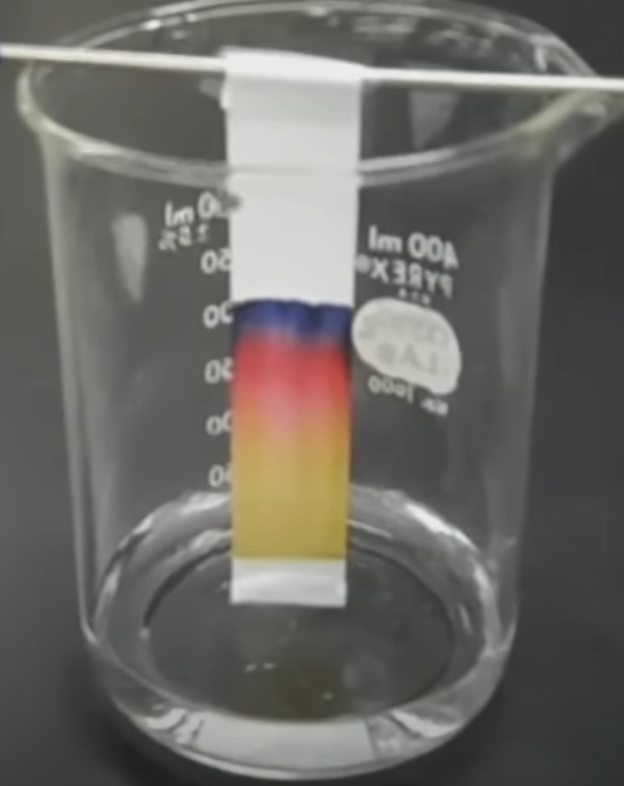
\includegraphics[height=0.3\textheight]{figures/纸层析法.png}
        \subcaption{化学实验中的纸层析法}
    \end{minipage}
    \begin{minipage}[c]{0.48\textwidth}
        \centering
        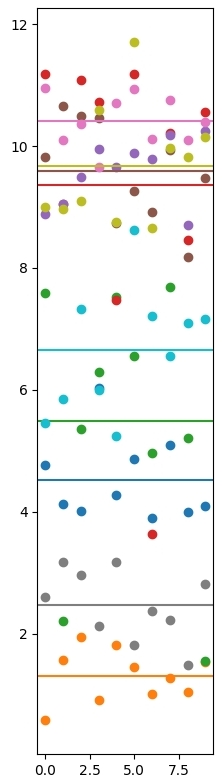
\includegraphics[height=0.3\textheight]{figures/1条滤纸.jpg}
        \subcaption{以 X 轴加速度的均值绘制的“滤纸条”}
    \end{minipage}
    \caption{“纸层析法”}
    \label{fig:滤纸条}
\end{figure}

我们同时将每一名志愿者的该项数字特征的 10 次测量值的均值绘制在滤纸条中,即对应颜色的横线。

直观地看,我们可以发现,同一名志愿者的每次运动的特征值的分布是相似的,而不同志愿者的特征值的分布则有一定的差异,
例如图中橙色的点大多集中在“滤纸”的底部,而粉色的点则大多集中在“滤纸”的顶部。
这说明不同的志愿者无论进行相同或是不同的动作,我们都可以通过比较这些数字特征来区分他们。

接下来我们对所有 $6 \times 8 = 48$ 种有量纲指标进行同样的“纸层析”操作,
得到了 48 张“滤纸条”,如\cref{fig:48条滤纸} 所示。
\cref{fig:48条滤纸} 中从上到下分别代表 X,Y,Z 轴加速度和 X,Y,Z 轴角速度 6 种测量对象,
从左到右依次为最大值、最小值、中位数、均值、方差、峰值、峰-峰值、有效值 8 中有量纲指标。

\begin{figure}[!htbp]
    \centering
    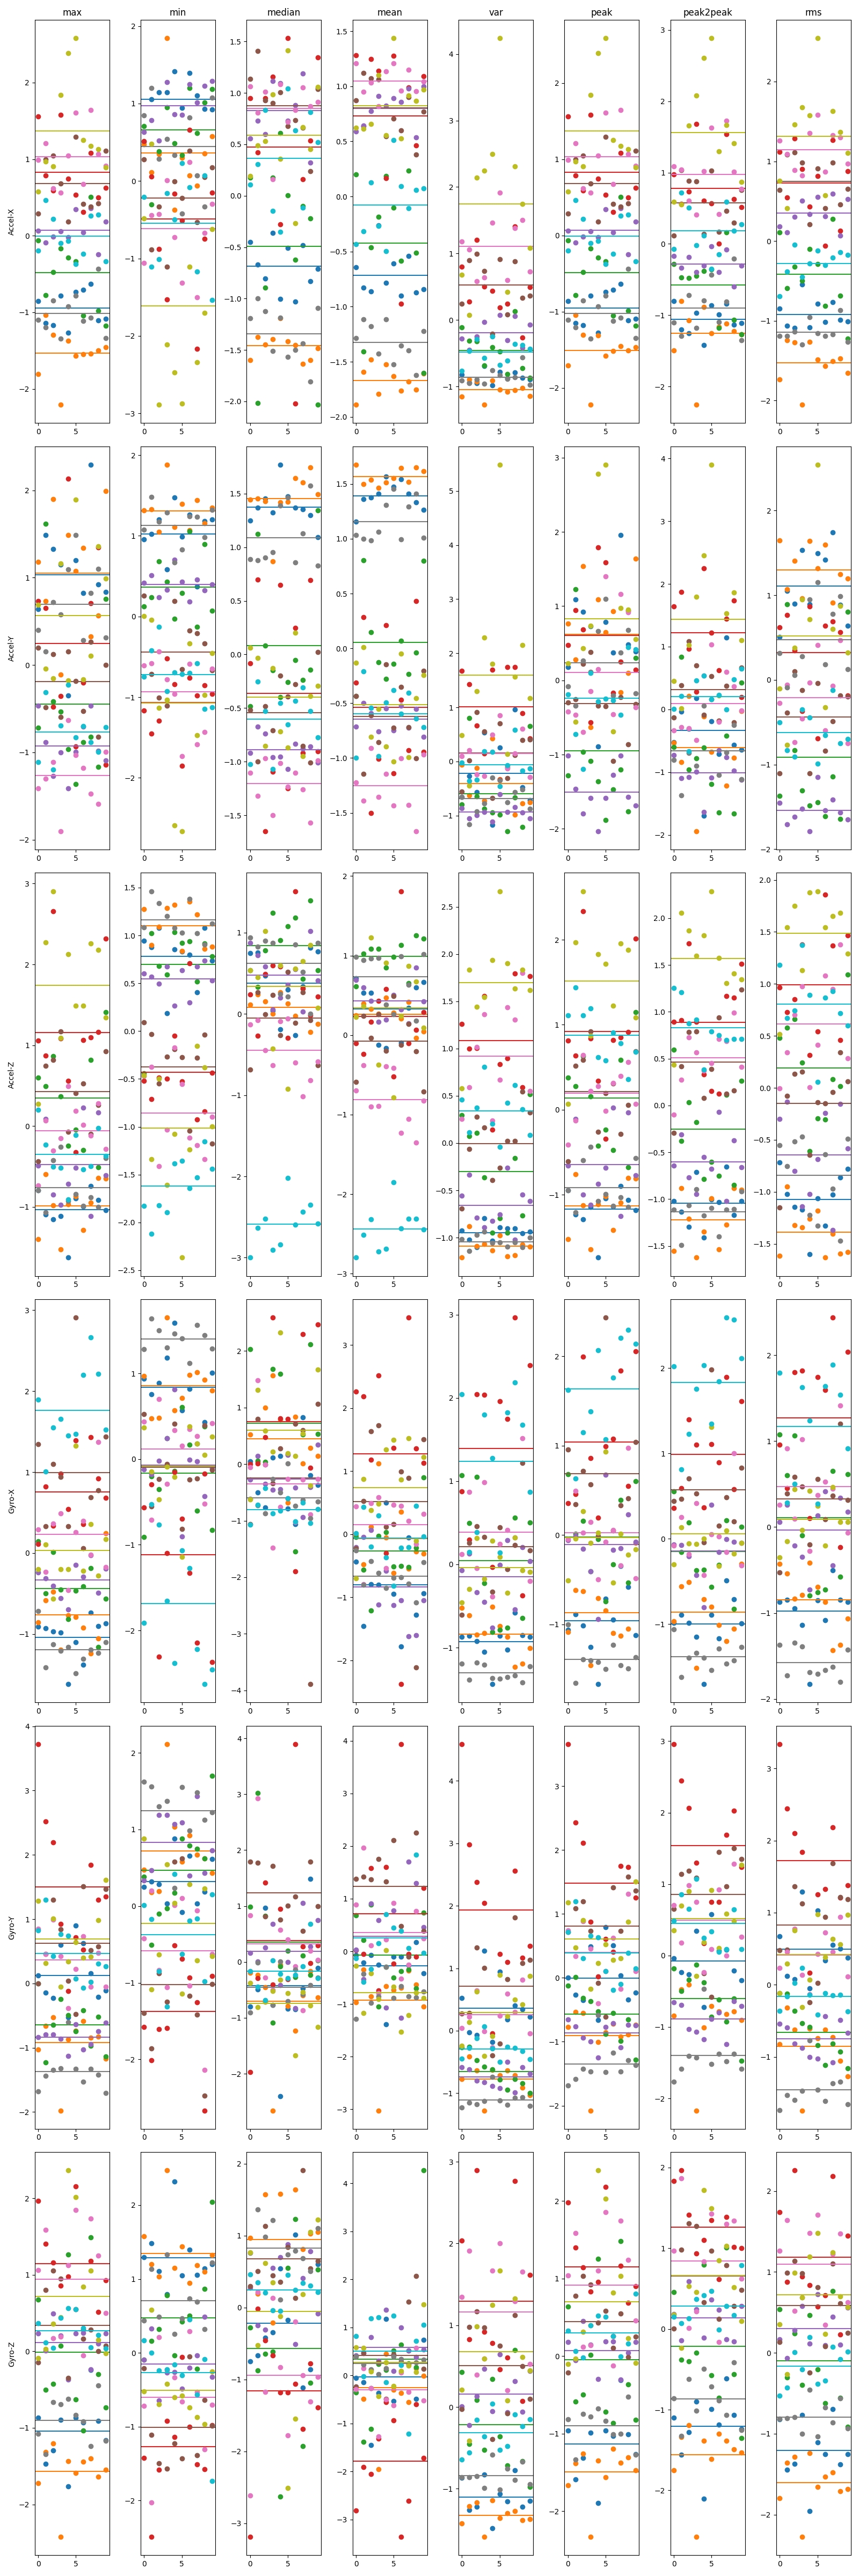
\includegraphics[width=0.5\textwidth]{figures/48条滤纸.jpg}
    \caption{48 张“滤纸条”}
    \label{fig:48条滤纸}
\end{figure}

但是,这 48 项数字特征中,肯定有某些特征的区分度更高,而某些特征的区分度更低。
因此我们在进行“指纹”的鉴定前,我们还需要对这些特征进行评估筛选。

\subsection{寻找代表“指纹”的特征}

我们同时用滤纸的方法对 $6 \times 6 = 36$ 种无量纲指标进行了可视化处理,但是发现它们的区分度并不高,因此不再对它们进行后续的分析。

\subsubsection{建立特征的评估标准}
\label{feature_evaluation}

为了量化地评估每一项特征的区分度,我们需要建立一套评估标准。

一张“滤纸条”如果能够很好地区分不同的志愿者,那么它应该具有以下特征:

\begin{enumerate}
    \item 每一名志愿者的 10 次实验的特征值的分布应该是相似的,即每一名志愿者的 10 个点应该尽可能地靠近一起。
    \item 不同志愿者的特征值的分布应该是不同的,即不同志愿者的 10 个点应该尽可能地分散开,而不是全部聚集在一片很小的区域内。
\end{enumerate}

其中,第 1 项特征可以用同一志愿者的 10 个样本点的\textbf{标准差}或者\textbf{峰峰值}来刻画。
标准差越小、峰峰值越小,就说明同一名志愿者的 10 个样本点越集中。
因此对于一条“滤纸”上的所有样本点,我们计算每一名志愿者的 10 个样本点的标准差,再取其平均值;
同时计算每一名志愿者的 10 个样本点的极差,再取其平均值。
二者加权求和,即可得到第 1 项特征的评估指标。

然而,最值、均值、方差、峰峰值这些数字特征的数量级并不相同,因此在计算评估指标前,我们还要把这些数据标准化。
\begin{equation}
    \label{eq:standardization}
    x_{ij} = \frac{x_{ij} - \mu_j}{\sigma_j}
\end{equation}

式 \cref{eq:standardization} 可以套用于任意数字特征中,将 $x_{ij}$ 标准化为 $x_{ij}$ 的标准分。
标准化完成后,我们就可以用下面的公式计算第 1 项特征的评估指标。

\begin{equation}
    \label{eq:feature-1}
    K_1 = \frac{w_{01}}{10} \sum_{i=1}^{10} \sigma_i + \frac{w_{02}}{10} \sum_{i=1}^{10} \left( \max_{j=1}^{10} x_{ij} - \min_{j=1}^{10} x_{ij} \right)
\end{equation}

式\cref{eq:feature-1} 中,$w_{01}$ 和 $w_{02}$ 是两项指标的权重,本文取 $w_{01} = 0.7$,$w_{02} = 0.3$。

第 2 项特征可以用不同志愿者的所有样本均值间的平均距离来刻画。
如果相邻样本间距离大,说明不同志愿者的样本点分散开,区分度高。
因此我们可以计算一张“滤纸条”上相邻横线间的平均距离,作为第 2 项特征的评估指标。

\begin{equation}
    \label{eq:feature-2}
    K_2 = \frac{1}{C_{10}^2} \sum_{i=1}^{9}\sum_{j=i+1}^{10} \left( \mu_{j} - \mu_{i} \right)
\end{equation}

在计算出所有特征的这两个指标后,我们最后再计算这两个指标的加权和,作为这条“滤纸条”的评估指标。
由于 $K_1$ 要求越小越好,$K_2$ 要求越大越好,因此 $K_1$ 的权重系数 $w_1$ 为负数,$K_2$ 的权重系数 $w_2$ 为正数。

\begin{equation}
    \label{eq:feature}
    K = w_1 K_1 + w_2 K_2
\end{equation}

本文取 $w_1 = - 0.8$,$w_2 = 0.2$。 
通过式 \cref{eq:feature},我们就可以计算出每一个滤纸条的评估指标 $K$,并且将所有的滤纸条按照 $K$ 的大小进行排序。

\subsubsection{特征的优先度排序和筛选}

根据上一小节建立的评估标准,我们对 48 项特征进行了排序,并选出了分数最高的前 12 项
(完整的排名见附录中的 \cref{appendix:feature-ranking})。

\begin{table}[!htbp]
    \centering
    \caption{特征的优先度排名(前 12 名)}
    \begin{tabular}{|c|c|c|c|c|}
        \hline
        排名 & 特征 & 指标 1 得分 & 指标 2 得分 & 总分 \\ \hline
        1 & Y 轴加速度-均值 & 1.09 & 1.12 & -0.64 \\ \hline
        2 & X 轴加速度-均值 & 1.20 & 1.15 & -0.73 \\ \hline
        3 & X 轴加速度-有效值 & 1.25 & 1.20 & -0.76 \\ \hline
        4 & Z 轴加速度-方差 & 1.35 & 1.17 & -0.85 \\ \hline
        5 & Y 轴加速度-中位数 & 1.39 & 1.11 & -0.89 \\ \hline
        6 & Z 轴加速度-最小值 & 1.46 & 1.16 & -0.94 \\ \hline
        7 & X 轴加速度-最大值 & 1.48 & 1.18 & -0.95 \\ \hline
        8 & Z 轴加速度-峰峰值 & 1.48 & 1.17 & -0.95 \\ \hline
        9 & Z 轴加速度-均值 & 1.44 & 0.99 & -0.95 \\ \hline
        10 & X 轴加速度-峰值 & 1.49 & 1.17 & -0.95 \\ \hline
        11 & X 轴加速度-方差 & 1.49 & 1.09 & -0.98 \\ \hline
        12 & Z 轴加速度-中位数 & 1.51 & 0.93 & -1.02 \\ \hline
    \end{tabular}
\end{table}

\subsection{对测试数据进行判定}

\subsubsection{测试数据的“指纹”比对}

筛选出了最有效的数字特征后,我们即可利用它们绘制测试数据的“指纹”。

重复\cref{imu_features_extraction} 的数据特征提取步骤,
然后将这些特征的样本点绘制到 12 条“滤纸条”上,如\cref{fig:指纹比对-36} 和\cref{fig:指纹比对-25}。

\begin{figure}[!htbp]
    \centering
    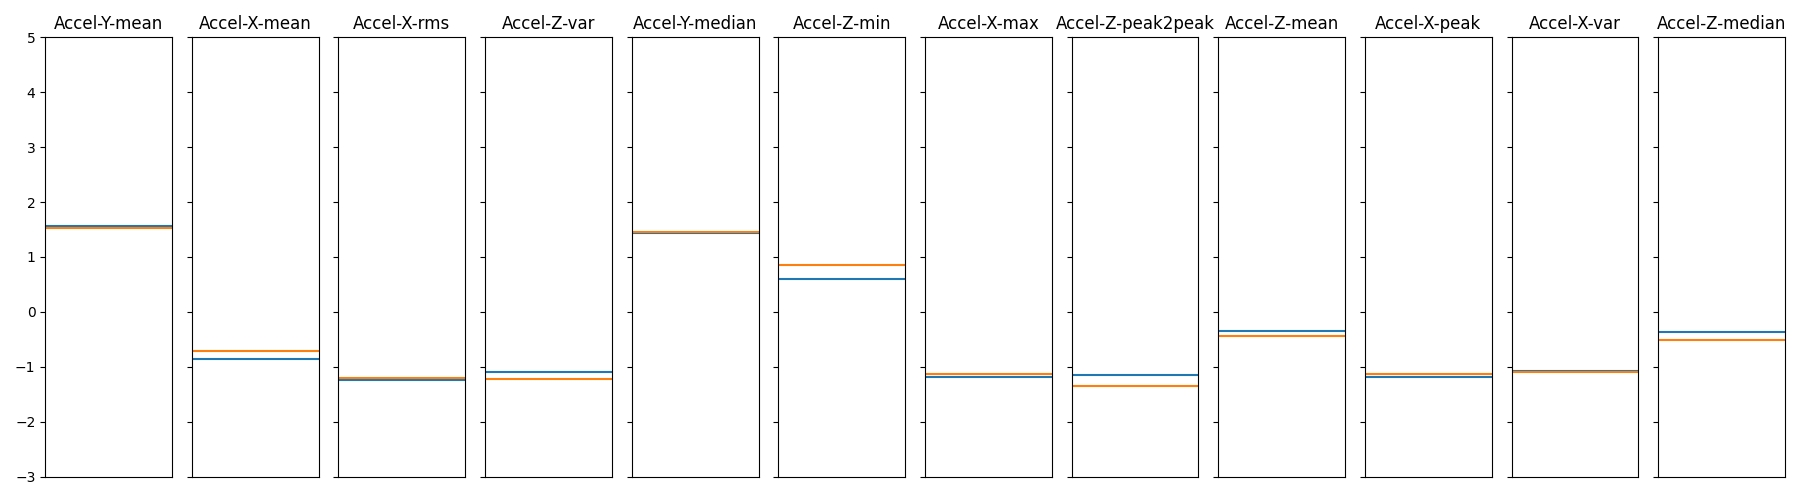
\includegraphics[width=\textwidth]{figures/指纹比对-35.jpg}
    \caption{测试数据对 36 的“指纹”对比}
    \label{fig:指纹比对-36}
\end{figure}

从\cref{fig:指纹比对-36} 可以直观地看出,该样本对的 12 个数据特征都彼此非常相似,因此我们可以认为它们来自同一个人。

\cref{fig:指纹比对-25} 是另外一个测试样本对,可以发现这一对的多数特征都有明显的差异,因此我们可以认为这 2 组运动数据来自不同的志愿者。

\begin{figure}[!htbp]
    \centering
    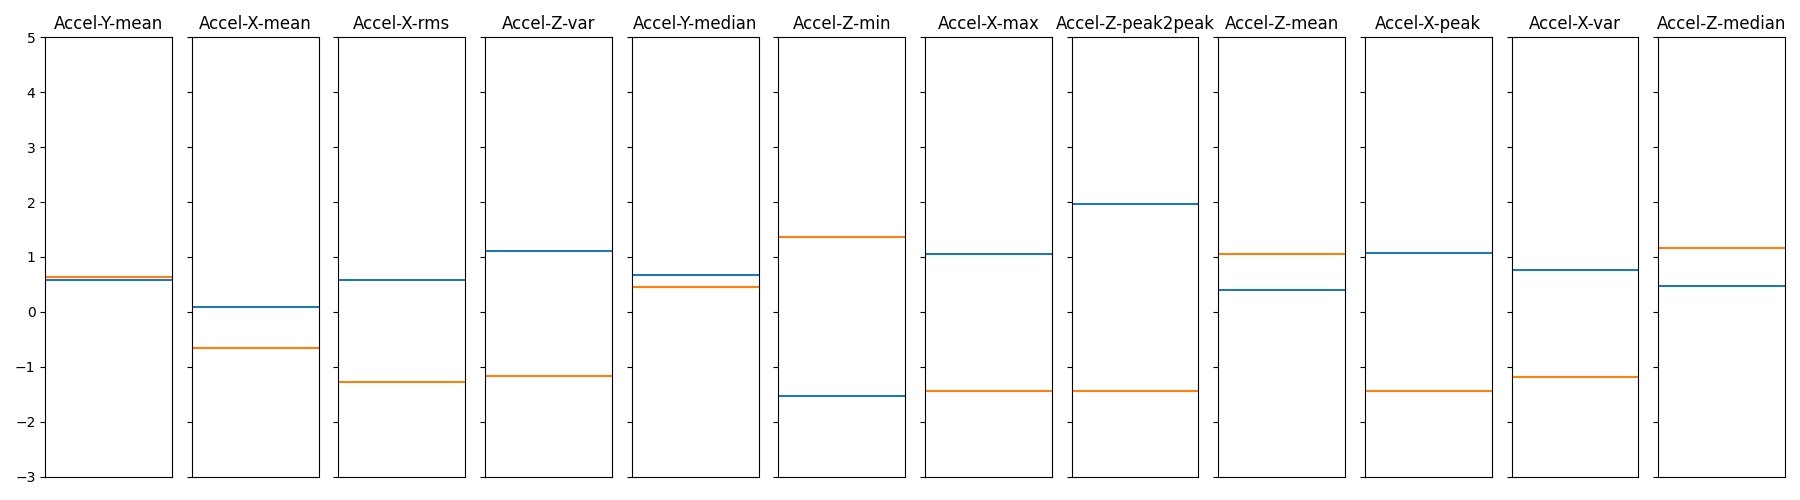
\includegraphics[width=\textwidth]{figures/指纹比对-24.jpg}
    \caption{测试数据对 25 的“指纹”对比}
    \label{fig:指纹比对-25}
\end{figure}

但是这仅代表两种比较理想的情况,实际上我们不能仅仅凭借主观的直觉来认定数据的身份一致性,因为还可能存在大量模棱两可的情况。
对此,我们需要采用一个算法,用数学判断身份的一致性。

\subsubsection{余弦相似度的计算}

用来描述两个向量的相似度的指标有很多,例如欧氏距离、曼哈顿距离、余弦相似度等。
本文采用了余弦相似度(Cosine Similarity)作为判断两组数据相似度的指标\cite{cosine-similarity}。

在有限维向量空间中,两个向量的方向如果越接近,则这两个向量之间的夹角越小,夹角的余弦值越大。

\begin{equation}
    \label{eq:cosine-similarity}
    \cos \theta = \frac{\vec{A} \cdot \vec{B}}{|\vec{A}| |\vec{B}|}
\end{equation}

这样就把两个向量之间的相似程度映射到了 $[-1, 1]$ 的区间内,越接近 1 说明越相似,越接近 -1 说明越不相似。
我们可以进一步通过线性变换将这个相似度映射到 $[0, 1]$ 区间内(见式 \cref{eq:cosine-similarity-probability}),
即可得出两个向量的相似概率。

\begin{equation}
    \label{eq:cosine-similarity-probability}
    P = \frac{1 + \cos \theta}{2}
\end{equation}

本文中,我们已经把每一对数据的特征浓缩为一对标准化的 12 维向量,
因此利用式 \cref{eq:cosine-similarity} 和 \cref{eq:cosine-similarity-probability},即可直接得出数据对的相似概率。

\subsubsection{身份一致性的判定}

计算出相似概率后,我们还需要确定一个阈值 $P_t$,来判断两组数据是否来自同一名志愿者。
如果概率大于阈值,则判断两组数据来自同一名志愿者,否则判断两组数据来自不同的志愿者。

为了确定这个阈值,我们利用参考数据集中的记录进行两两配对生成测试用例,以模型的正确率作为反馈,上下调整 $P_t$,最终确定
$P_t$ 的值为 0.90,此时参考数据测试的正确率为 87.08\%。

以上工作全部完成后,我们得出了测试数据集的最终判断结果,如\cref{tab:测试数据对判定结果}:

\begin{longtable}[!htbp]{|c|c|c|c|c|c|c|c|}
    \caption{测试数据对判定结果} \label{tab:测试数据对判定结果} \\
    \hline
    编号 & $\cos \theta$ & $P$ & 是否身份一致 & 编号 & $\cos \theta$ & $P$ & 是否身份一致 \\ \hline
    \endfirsthead
    \multicolumn{8}{c}{{\tablename\ \thetable{} -- 续前页}} \\ \hline
    编号 & $\cos \theta$ & $P$ & 是否身份一致 & 编号 & $\cos \theta$ & $P$ & 是否身份一致 \\ \hline
    \endhead
    \hline
    \multicolumn{8}{r}{{续下页}} \\ \hline
    \endfoot

    \endlastfoot
        1 & 0.97 & 0.986 & 是 & 51 & 0.97 & 0.986 & 是 \\ \hline 
        2 & 0.94 & 0.971 & 是 & 52 & -0.03 & 0.486 & 否 \\ \hline
        3 & 0.98 & 0.988 & 是 & 53 & 0.91 & 0.953 & 是 \\ \hline
        4 & 0.68 & 0.838 & 否 & 54 & 0.98 & 0.989 & 是 \\ \hline
        5 & 0.18 & 0.588 & 否 & 55 & 0.43 & 0.713 & 否 \\ \hline
        6 & 0.84 & 0.921 & 是 & 56 & 0.87 & 0.936 & 是 \\ \hline
        7 & 0.75 & 0.875 & 否 & 57 & -0.39 & 0.304 & 否 \\ \hline
        8 & 0.95 & 0.973 & 是 & 58 & -0.50 & 0.248 & 否 \\ \hline
        9 & 0.98 & 0.992 & 是 & 59 & 0.99 & 0.995 & 是 \\ \hline
        10 & 0.91 & 0.953 & 是 & 60 & 0.59 & 0.793 & 否 \\ \hline
        11 & -0.82 & 0.092 & 否 & 61 & 0.94 & 0.971 & 是 \\ \hline
        12 & 0.98 & 0.988 & 是 & 62 & 0.97 & 0.986 & 是 \\ \hline
        13 & 0.85 & 0.924 & 是 & 63 & 0.80 & 0.900 & 否 \\ \hline
        14 & 0.77 & 0.884 & 否 & 64 & 0.32 & 0.660 & 否 \\ \hline
        15 & 0.19 & 0.597 & 否 & 65 & 0.46 & 0.728 & 否 \\ \hline
        16 & 0.96 & 0.978 & 是 & 66 & 0.94 & 0.968 & 是 \\ \hline
        17 & 0.69 & 0.843 & 否 & 67 & 0.98 & 0.990 & 是 \\ \hline
        18 & -0.67 & 0.163 & 否 & 68 & 0.35 & 0.675 & 否 \\ \hline
        19 & 0.93 & 0.966 & 是 & 69 & -0.46 & 0.269 & 否 \\ \hline
        20 & 0.84 & 0.919 & 是 & 70 & -0.18 & 0.409 & 否 \\ \hline
        21 & 0.19 & 0.595 & 否 & 71 & 0.95 & 0.977 & 是 \\ \hline
        22 & 0.53 & 0.763 & 否 & 72 & 0.82 & 0.908 & 是 \\ \hline
        23 & 0.97 & 0.984 & 是 & 73 & 0.97 & 0.983 & 是 \\ \hline
        24 & 0.97 & 0.985 & 是 & 74 & 0.85 & 0.927 & 是 \\ \hline
        25 & -0.68 & 0.160 & 否 & 75 & 0.99 & 0.995 & 是 \\ \hline
        26 & 0.89 & 0.947 & 是 & 76 & 0.95 & 0.974 & 是 \\ \hline
        27 & 0.99 & 0.994 & 是 & 77 & 0.96 & 0.978 & 是 \\ \hline
        28 & 0.66 & 0.828 & 否 & 78 & 0.94 & 0.970 & 是 \\ \hline
        29 & -0.79 & 0.105 & 否 & 79 & 0.99 & 0.996 & 是 \\ \hline
        30 & -0.35 & 0.323 & 否 & 80 & 0.87 & 0.936 & 是 \\ \hline
        31 & 0.43 & 0.716 & 否 & 81 & -0.88 & 0.060 & 否 \\ \hline
        32 & 0.98 & 0.991 & 是 & 82 & 0.95 & 0.973 & 是 \\ \hline
        33 & 0.93 & 0.966 & 是 & 83 & 0.48 & 0.738 & 否 \\ \hline
        34 & 0.97 & 0.986 & 是 & 84 & 0.44 & 0.722 & 否 \\ \hline 
        35 & 0.04 & 0.521 & 否 & 85 & -0.08 & 0.462 & 否 \\ \hline
        36 & 0.99 & 0.997 & 是 & 86 & 0.86 & 0.930 & 是 \\ \hline
        37 & -0.47 & 0.266 & 否 & 87 & 0.72 & 0.861 & 否 \\ \hline
        38 & 0.96 & 0.978 & 是 & 88 & 0.96 & 0.979 & 是 \\ \hline
        39 & 0.52 & 0.762 & 否 & 89 & -0.46 & 0.268 & 否 \\ \hline
        40 & -0.24 & 0.379 & 否 & 90 & 0.51 & 0.756 & 否 \\ \hline
        41 & 0.95 & 0.974 & 是 & 91 & 0.37 & 0.686 & 否 \\ \hline
        42 & -0.24 & 0.379 & 否 & 92 & 0.86 & 0.928 & 是 \\ \hline
        43 & 0.59 & 0.794 & 否 & 93 & -0.73 & 0.134 & 否 \\ \hline
        44 & 0.06 & 0.531 & 否 & 94 & 0.99 & 0.997 & 是 \\ \hline
        45 & -0.66 & 0.170 & 否 & 95 & 0.70 & 0.852 & 否 \\ \hline
        46 & 0.73 & 0.867 & 否 & 96 & 0.89 & 0.946 & 是 \\ \hline
        47 & 0.45 & 0.724 & 否 & 97 & 0.12 & 0.561 & 否 \\ \hline
        48 & 0.91 & 0.957 & 是 & 98 & -0.72 & 0.142 & 否 \\ \hline
        49 & 0.85 & 0.926 & 是 & 99 & 0.89 & 0.947 & 是 \\ \hline
        50 & 0.87 & 0.936 & 是 & 100 & 0.91 & 0.957 & 是 \\ \hline
\end{longtable}

100 个样本数据对中,共有 52 组被判定为来自同一名志愿者,48 组被判定为来自不同的志愿者。

\section{模型的检验}

为了确定前文中的阈值 $P_t$,我们已经使用参考数据集对判断模型进行了测试,其正确率为 87.08\%。

我们也可以通过直观的观察来判断模型的正确性。
例如\cref{fig:指纹比对-36} 从直接的视觉效果上看,两组数据的“指纹图谱”是非常接近的,
而在\cref{tab:测试数据对判定结果} 中,第 36 组的相似概率达到了 0.997;
\cref{fig:指纹比对-25} 中大多数“滤纸条”上的数据都有明显的差异,
\cref{tab:测试数据对判定结果} 中,第 25 组的相似概率只有 0.160。

因此,我们可以初步认为本文提出的模型是有效的。

\section{模型的优缺点分析}
\label{pros-and-cons}

\subsection{本模型的优点}

\begin{enumerate}
    \item 对数据的依赖性低。不同于神经网络训练需要大量的数据
    (这里的“大量”指的是样本个数而不是时间序列的长度),
    本文的指纹图谱模型在仅有 100 份参考数据的情况下,仍然能高效地提取出主要的数字特征。
    即使参考数据的时间序列更短,本模型也不会受到非常大的影响。
    \item 结构简洁直观。相比神经网络无法得知其内部的运算逻辑,本模型的每一个步骤都是可解释的。
    \item 运算量低,效率高。本文通过建立评价体系筛序主要数字特征有效地对数据进行了降维,
    在保证正确率的前提下兼顾了运算速度。
    由于没有引入神经网络等人工智能算法,因此本模型对计算机性能的要求很低,可以广泛部署到智能穿戴设备中。
\end{enumerate}

\subsection{本模型的缺点}

\begin{enumerate}
    \item 人工干涉的过程太多。本模型建立特征评估标准时的权重、筛选出的主要特征个数都是人为规定的,
    这导致权重的选择直接影响了特征的评分和排名,有可能所得的并不是最佳的筛选结果。
    事实上,这一个步骤应有对应的模型或算法来自动完成,否则会降低模型的说服力。
    \item 本模型面对类别过多的复杂数据集时解释性可能会下降,当两个类别在我们选取的特征中不相似的特征维度较少时,判断的准确性不高。
\end{enumerate}

\section{模型的改进与推广}

基于上一节的分析,本模型可以针对主要特征的筛选步骤进行改进,
即考虑引入具备自适应能力的新模型,如一些深度学习模型,用来实现评制定价标准环节权重参数的自动调节,和主要特征的自动筛选,以更好地捕捉输入与特征之间的复杂关系,减少计算中的人工成分。

\bigskip

本模型除了用于识别 IMU 运动数据的身份一致性,还可以推广到更多的应用场景中。

\subsection{应用于域内样本识别}
本模型虽然针对的是域外样本的生物识别,但“指纹图谱”本身其实可以被保存下来,作为未来判断身份的依据。
也就是说,本模型除了用来判断陌生样本的身份一致性以外,还可以用来将陌生样本与“指纹库”中保存的指纹信息进行比对,找出陌生样本是否属于该库,或者属于已知的哪个用户。

\subsection{从其他来源中提取特征}
运动数据的来源除了惯性传感器,还可以是机器视觉捕捉到的图像等。
从图像对人体骨架进行识别,可以重建人的三维运动过程。
此时我们即可利用本文的模型从这个三维的运动过程中提取出主要的运动特征,
实现对人体步态等多种关节运动的识别判断。

\begin{thebibliography}{9} % 参考文献
    \bibitem[1]{1021136457.nh}
    谭智豪.
    \newblock 基于移动设备使用行为的身份认证研究[D].
    \newblock 北京邮电大学, 2022.
    \bibitem[2]{cosine-similarity}
    P.-N. Tan, M. Steinbach \& V. Kumar.
    \newblock "Introduction to Data Mining".
    \newblock Addison-Wesley, 2005.
    \newblock ISBN 0-321-32136-7.
    \newblock Chapter 8.
\end{thebibliography}

\newpage

\begin{appendices} % 附录

\section{完整的特征评价指标排名}
\label{appendix:feature-ranking}

\begin{longtable}{|c|c|c|c|c|}
    \hline
    排名 & 特征 & 指标 1 得分(越小越好) & 指标 2 得分(越大越好) & 总分 \\ \hline
    \endfirsthead
    \multicolumn{5}{c}{{\tablename\ \thetable{} -- 续前页}} \\
    \hline
    排名 & 特征 & 指标 1 得分(越小越好) & 指标 2 得分(越大越好) & 总分 \\ \hline
    \endhead
    \hline
    \multicolumn{5}{r}{{续下页}} \\
    \endfoot
    \hline
    \endlastfoot
    1 & Accel-Y-mean & 1.09 & 1.12 & -0.64 \\ \hline
    2 & Accel-X-mean & 1.20 & 1.15 & -0.73 \\ \hline
    3 & Accel-X-rms & 1.25 & 1.20 & -0.76 \\ \hline
    4 & Accel-Z-var & 1.35 & 1.17 & -0.85 \\ \hline
    5 & Accel-Y-median & 1.39 & 1.11 & -0.89 \\ \hline
    6 & Accel-Z-min & 1.46 & 1.16 & -0.94 \\ \hline
    7 & Accel-X-max & 1.48 & 1.18 & -0.95 \\ \hline
    8 & Accel-Z-peak2peak & 1.48 & 1.17 & -0.95 \\ \hline
    9 & Accel-Z-mean & 1.44 & 0.99 & -0.95 \\ \hline
    10 & Accel-X-peak & 1.49 & 1.17 & -0.95 \\ \hline
    11 & Accel-X-var & 1.49 & 1.09 & -0.98 \\ \hline
    12 & Accel-Z-median & 1.51 & 0.93 & -1.02 \\ \hline
    13 & Accel-Y-min & 1.59 & 1.13 & -1.04 \\ \hline
    14 & Accel-Z-rms & 1.64 & 1.17 & -1.08 \\ \hline
    15 & Accel-X-peak2peak & 1.64 & 1.15 & -1.08 \\ \hline
    16 & Gyro-Z-rms & 1.65 & 1.14 & -1.09 \\ \hline
    17 & Gyro-Z-var & 1.73 & 1.11 & -1.16 \\ \hline
    18 & Gyro-Y-rms & 1.75 & 1.12 & -1.17 \\ \hline
    19 & Gyro-X-peak2peak & 1.78 & 1.13 & -1.20 \\ \hline
    20 & Gyro-Y-var & 1.78 & 1.04 & -1.22 \\ \hline
    21 & Accel-X-median & 1.83 & 1.05 & -1.26 \\ \hline
    22 & Gyro-Z-peak2peak & 1.86 & 1.11 & -1.27 \\ \hline
    23 & Gyro-X-max & 1.87 & 1.13 & -1.27 \\ \hline
    24 & Accel-Z-peak & 1.87 & 1.11 & -1.27 \\ \hline
    25 & Gyro-X-rms & 1.89 & 1.07 & -1.30 \\ \hline
    26 & Accel-Y-rms & 1.92 & 1.08 & -1.32 \\ \hline
    27 & Gyro-X-var & 1.93 & 1.04 & -1.34 \\ \hline
    28 & Gyro-X-min & 1.95 & 1.05 & -1.35 \\ \hline
    29 & Gyro-X-peak & 1.97 & 1.10 & -1.36 \\ \hline
    30 & Gyro-Y-peak2peak & 1.97 & 1.10 & -1.36 \\ \hline
    31 & Gyro-Z-peak & 1.98 & 1.06 & -1.37 \\ \hline
    32 & Accel-Z-max & 1.99 & 1.08 & -1.38 \\ \hline
    33 & Gyro-Z-max & 1.99 & 1.06 & -1.38 \\ \hline
    34 & Gyro-Y-max & 2.06 & 1.07 & -1.43 \\ \hline
    35 & Gyro-Y-peak & 2.14 & 1.07 & -1.49 \\ \hline
    36 & Gyro-Z-min & 2.24 & 1.09 & -1.57 \\ \hline
    37 & Accel-X-min & 2.38 & 0.99 & -1.70 \\ \hline
    38 & Accel-Y-max & 2.43 & 1.01 & -1.74 \\ \hline
    39 & Gyro-Y-min & 2.45 & 1.03 & -1.76 \\ \hline
    40 & Accel-Y-var & 2.43 & 0.89 & -1.77 \\ \hline
    41 & Accel-Y-peak2peak & 2.59 & 0.95 & -1.88 \\ \hline
    42 & Accel-Y-peak & 2.83 & 0.87 & -2.09 \\ \hline
    43 & Gyro-Z-median & 2.91 & 0.87 & -2.15 \\ \hline
    44 & Gyro-X-mean & 2.97 & 0.82 & -2.22 \\ \hline
    45 & Gyro-Y-mean & 3.07 & 0.84 & -2.29 \\ \hline
    46 & Gyro-Z-mean & 3.05 & 0.70 & -2.30 \\ \hline
    47 & Gyro-X-median & 3.34 & 0.67 & -2.54 \\ \hline
    48 & Gyro-Y-median & 3.43 & 0.71 & -2.60 \\ \hline
\end{longtable}

\section{参考数据绘图程序 - Python}

\begin{lstlisting}[language=python]
import numpy as np
import matplotlib.pyplot as plt

# 读取数据
dataType = 'reference'
subject = '1'
trial = '4'

fileName = f'code\\{dataType}\\{subject}\\{trial}.txt'
df = np.loadtxt(fileName)

# 折线图
fig, axs = plt.subplots(nrows=2, ncols=1, figsize=(10, 4))
fig.suptitle(f'{dataType} {subject}-{trial}')
subtitles = ['Accel', 'Gyro']
Axes = ['X','Y','Z']
for i in range(2):
    for j in range(3):
        x = np.arange(df.shape[1])
        y = df[3*i+j, :]
        axs[i].plot(x, y, label=Axes[j])
    axs[i].set_title(subtitles[i])
plt.tight_layout()
plt.legend()
plt.savefig(f'code\\images\\{dataType}-{subject}-{trial}.png')
plt.show()

# 箱型图
fig, ax = plt.subplots(figsize=(7, 5))
fig.suptitle(f'{dataType} {subject}-{trial}')
ax.boxplot(df.T, labels=[f'{i+1}' for i in range(df.shape[0])])
plt.savefig(f'code\\images\\{dataType}-{subject}-{trial}-boxplot.png')
plt.show()
\end{lstlisting}

\section{卡尔曼滤波算法 - Python}

\begin{lstlisting}[language=python]
import numpy as np
import matplotlib.pyplot as plt
import os
import csv

class Kalman_Filter:
    def __init__(self, Q, R): # 构造函数
        self.Q = Q
        self.R = R

        self.P_k_k1 = 1
        self.Kg = 0
        self.P_k1_k1 = 1
        self.x_k_k1 = 0
        self.ADC_OLD_Value = 0
        self.Z_k = 0
        self.kalman_adc_old=0

    def Kalman(self, ADC_Value):
        self.Z_k = ADC_Value

        if ( abs(self.kalman_adc_old - ADC_Value) >= 60 ):
            self.x_k1_k1 = ADC_Value * 0.382 + self.kalman_adc_old * 0.618
        else:
            self.x_k1_k1 = self.kalman_adc_old

        self.x_k_k1 = self.x_k1_k1
        self.P_k_k1 = self.P_k1_k1 + self.Q
        self.Kg = self.P_k_k1 / (self.P_k_k1 + self.R)

        kalman_adc = self.x_k_k1 + self.Kg * (self.Z_k - self.kalman_adc_old)
        self.P_k1_k1 = (1 - self.Kg) * self.P_k_k1
        self.P_k_k1 = self.P_k1_k1

        self.kalman_adc_old = kalman_adc
        return kalman_adc

def GetSampleTime(timelist):
    "获取时间列表的平均取样时间间隔"
    sampleNum = len(timelist)
    timeInterval = [timelist[j+1] - timelist[j] for j in range(0, sampleNum-1)]
    _timeInterval = np.asarray(timeInterval)
    avgSampleTime = np.mean(_timeInterval)
    return avgSampleTime

if __name__ == '__main__':
    number = ['1','2','3','4','5','6','7','8','9','10']
    for i in range(1,11):
        for j in range(1,11):
            # 读取数据
            dataType = 'reference'
            subject = number[i-1]
            trial = number[j-1]

            fileName = f'code\\{dataType}\\{subject}\\{trial}.txt'
            df = np.loadtxt(fileName)
            
            time0 = list(range(1, df.shape[1] + 1)) # 时间节点
            time = [x * 0.002 for x in time0]
            accx = df[0].tolist() # x轴加速度
            accy = df[1].tolist() # y轴加速度
            accz = df[2].tolist() # z轴加速度
            gyrox = df[3].tolist() # x轴角速度
            gyroy = df[4].tolist() # y轴角速度
            gyroz = df[5].tolist() # z轴角速度
            
            # 卡尔曼滤波
            AccX_Filter = Kalman_Filter(0.001, 0.1)
            AccY_Filter = Kalman_Filter(0.001, 0.1)
            AccZ_Filter = Kalman_Filter(0.001, 0.1)
            GyroX_Filter = Kalman_Filter(0.001, 0.1)
            GyroY_Filter = Kalman_Filter(0.001, 0.1)
            GyroZ_Filter = Kalman_Filter(0.001, 0.1)

            sampleTime = GetSampleTime(time)
            sampleNum = len(time)
            timeAxis = np.linspace(0, sampleNum*sampleTime, sampleNum, True)

            filteredAccX = []
            filteredAccY = []
            filteredAccZ = []
            filteredGyroX = []
            filteredGyroY = []
            filteredGyroZ = []
            for k in range (0, sampleNum):
                filteredAccX.append(AccX_Filter.Kalman(accx[k]))
                filteredAccY.append(AccY_Filter.Kalman(accy[k]))
                filteredAccZ.append(AccZ_Filter.Kalman(accz[k]))
                filteredGyroX.append(GyroX_Filter.Kalman(gyrox[k]))
                filteredGyroY.append(GyroY_Filter.Kalman(gyroy[k]))
                filteredGyroZ.append(GyroZ_Filter.Kalman(gyroz[k]))
                
            df1 = np.array([filteredAccX,filteredAccY,filteredAccZ,filteredGyroX,filteredGyroY,filteredGyroZ])
            
            folder1 = 'code\\referenceKalman'
            folder2 = subject
            file_name = f'{trial}.txt'
      
            path1 = os.path.join(folder1, folder2)
            if not os.path.exists(path1):
                os.makedirs(path1)
            path2 = os.path.join(path1, file_name)
            np.savetxt(path2,df1)
\end{lstlisting}

\section{提取时序特征程序 - Python}

\begin{lstlisting}[language=python]
import numpy as np
from scipy.stats import kurtosis, skew

def get_features(y):
    """
    Args:
        y : wave data
    Returns:
        max_y(最大值), min_y(最小值), median_y(中位数), mean_y(均值), var_y(方差), peak(峰值), peak2peak(峰峰值), rms(有效值),
        crestf(峰值因子), margin(裕度因子), pulse(脉冲因子), waveform(波形因子), kur(峭度因子), sk(偏度因子)
    """
    max_y = np.max(y)
    min_y = np.min(y)
    median_y = np.median(y)
    mean_y = np.mean(y)
    var_y = np.var(y)
 
    rms = np.sqrt(np.mean(np.square(y)))
    peak = max(abs(max_y), abs(min_y))
    peak2peak = max_y - min_y
    # 峰值因子
    crestf = max_y / rms if rms != 0 else 0
    xr = np.square(np.mean(np.sqrt(np.abs(y))))
    # 裕度
    margin = (max_y / xr) if xr != 0 else 0 
    yr = np.mean(np.abs(y))
    # 脉冲因子
    pulse = max_y / yr if yr != 0 else 0 
    # 波形因子
    waveform = rms / yr if yr !=0 else 0  
    # 峭度
    kur = kurtosis(y) 
    # 偏斜度
    sk = skew(y)   
    #[max_y, min_y, median_y, mean_y, var_y, peak, peak2peak, rms, crestf, margin, pulse,waveform, kur, sk]
    features = np.array([max_y, min_y, median_y, mean_y, var_y, peak, peak2peak, rms]) 
    return features
    
data = []

for i in range(100):
    dataType = 'test'
    subject = i+1
    fileName = f'code\\{dataType}\\{subject}\\a.txt'
    df = np.loadtxt(fileName)
    feature_v = np.array([get_features(df[0]),get_features(df[1]),get_features(df[2]),get_features(df[3]),get_features(df[4]),get_features(df[5])]).flatten()
    data.append(feature_v)
    fileName = f'code\\{dataType}\\{subject}\\b.txt'
    df = np.loadtxt(fileName)
    feature_v = np.array([get_features(df[0]),get_features(df[1]),get_features(df[2]),get_features(df[3]),get_features(df[4]),get_features(df[5])]).flatten()
    data.append(feature_v)
data1 = np.array(data)
print(data1.shape)
np.savetxt("code\\testreference.txt",data1)
\end{lstlisting}

\section{“滤纸条”绘图程序 - Python}

\begin{lstlisting}[language=python]
import numpy as np
import matplotlib.pyplot as plt
from pyparsing import col

fileName = f'code\\reference1.txt'
df = np.loadtxt(fileName)

df = (df - np.mean(df, axis=0)) / np.std(df, axis=0)

colors = plt.rcParams['axes.prop_cycle'].by_key()['color'][:10]
fig, axs = plt.subplots(nrows=6, ncols=8, figsize=(16, 48))
x = np.arange(10)
xtitile = ['max', 'min', 'median', 'mean', 'var', 'peak', 'peak2peak', 'rms']
ytitile = ['Accel-X','Accel-Y','Accel-Z','Gyro-X','Gyro-Y','Gyro-Z']
for j in range(8):
    axs[0][j].set_title(xtitile[j])
for j in range(6):
    axs[j][0].set_ylabel(ytitile[j])
for k in range(6):
    for j in range(8):
        for i in range(10):
            y = (df.T)[8*k+j]
            z = y[i*10:i*10+10]
            axs[k][j].plot(x,z,'o',color=colors[i])
            axs[k][j].axhline(z.mean(),color=colors[i])
plt.tight_layout()
plt.savefig(f'code\\images\\features-1-normalized.png')
plt.show()
\end{lstlisting}

\section{特征优先度排序程序 - Python}

\begin{lstlisting}[language=python]
import numpy as np

fileName = f'code\\reference1.txt'
df = np.loadtxt(fileName)  # 100*48
df = (df - np.mean(df, axis=0)) / np.std(df, axis=0)

w1 = -0.8
w2 = 0.2

k1 = np.zeros(48)
k2 = np.zeros(48)

vector_names = ['' for _ in range(48)]
xtitile = ['max', 'min', 'median', 'mean', 'var', 'peak', 'peak2peak', 'rms']
ytitile = ['Accel-X', 'Accel-Y', 'Accel-Z', 'Gyro-X', 'Gyro-Y', 'Gyro-Z']

for i in range(6):
    for j in range(8):
        ave = np.zeros(10)
        y = (df.T)[8 * i + j]
        for k in range(10):
            z = y[k * 10:k * 10 + 10]
            ave[k] = z.mean()
            k1[8 * i + j] += np.std(z, axis=0) / 10 + (np.max(z, axis=0) - np.min(z, axis=0)) / 10
        for ii in range(9):
            for jj in range(ii+1,10):
                k2[8 * i + j] += np.abs(ave[ii] - ave[jj])/45

        # 命名每个向量
        vector_names[8 * i + j] = f'{ytitile[i]}-{xtitile[j]}'

num = np.arange(48)
# 创建一个包含向量名称和分数的列表
score_list = list(zip(vector_names, k1, k2, num, w1 * k1 + w2 * k2))

# 对列表根据分数进行排序
sorted_scores = sorted(score_list, key=lambda x: x[4], reverse=True)

# 打印排序后的向量名称、排名和分数
for rank, (name, k1_value, k2_value, num1, score) in enumerate(sorted_scores, start=1):
    print(f'{rank} & {name} & {k1_value:.2f} & {k2_value:.2f} & {score:.2f} \\\\ \\hline')
\end{lstlisting}

\section{测试数据判定程序 - Python}

\begin{lstlisting}[language=python]
import numpy as np
import matplotlib.pyplot as plt
import torch.nn as nn
import torch

def map_cosine_similarity_to_0_1(cosine_similarity):
    return (cosine_similarity + 1) / 2

# 读取数据
df = np.loadtxt('code\\testreference.txt')
num = [11,3,7,20,10,17,0,22,19,5,4,18]


fileName = f'code\\reference1.txt'
df1 = np.loadtxt(fileName)  # 100*48
df = (df - np.mean(df1, axis=0)) / np.std(df1, axis=0)
df1 = (df1 - np.mean(df1, axis=0)) / np.std(df1, axis=0)

colors = plt.rcParams['axes.prop_cycle'].by_key()['color'][:10]

name = ['Accel-Y-mean','Accel-X-mean','Accel-X-rms','Accel-Z-var','Accel-Y-median','Accel-Z-min','Accel-X-max','Accel-Z-peak2peak','Accel-Z-mean','Accel-X-peak','Accel-X-var','Accel-Z-median']

data = df[:,num]
data1 = df1[:,num]

for i in range(100):
    fig, axs = plt.subplots(nrows=1, ncols=12, figsize=(18, 5), sharey=True)
    for j in range(12):
        axs[j].set_title(name[j])
        axs[j].axhline(np.array([data[2*i,j]]),color=colors[0])
        axs[j].axhline(np.array([data[2*i+1,j]]),color=colors[1])
        axs[j].tick_params(axis='x', which='both', bottom=False, top=False, labelbottom=False)  # 隐藏 x 轴刻度
        axs[j].set_ylim(-3, 5)  # 设置 y 轴范围
    plt.tight_layout()
    plt.savefig(f'code\\images\\test-features-{i}.png')

for i in range(100):
    input1 = torch.Tensor(data[2*i]).unsqueeze(0)
    input2 = torch.Tensor(data[2*i+1]).unsqueeze(0)
    cos = nn.CosineSimilarity(dim=1, eps=1e-6)
    output = cos(input1, input2).item()
    if map_cosine_similarity_to_0_1(output) > 0.9:
        flag = '是'
    else:
        flag = '否'
    print(f'{i+1} & {output:.2f} & {map_cosine_similarity_to_0_1(output):.3f} & {flag} \\\\ \\hline ')
    
cnt = 0
for i in range(100):
    for j in range(100):
        input1 = torch.Tensor(data1[i]).unsqueeze(0)
        input2 = torch.Tensor(data1[j]).unsqueeze(0)
        cos = nn.CosineSimilarity(dim=1, eps=1e-6)
        output = cos(input1, input2).item()
        output = map_cosine_similarity_to_0_1(output)
        if i//10 == j//10:
            #color1 = colors[0]
            if output > 0.9:
                cnt += 1
        else:
            #color1 = colors[1]
            if output <= 0.9:
                cnt += 1
        #plt.plot(np.array([i%10]),np.array([output]),'o',color=color1)
#plt.show()
print(cnt/10000)
\end{lstlisting}

\end{appendices}

\end{document} 